\documentclass{article}
%\usepackage{icml2014} 
\usepackage[accepted]{icml2014}
\usepackage{times}
\usepackage{graphicx}
%\usepackage{mdwlist}
\usepackage{bbm}
\usepackage{microtype}
\usepackage{color}
\usepackage{natbib}
%\usepackage{todonotes}
\usepackage{algorithm}
\usepackage{algorithmic}
\usepackage{multirow}
\usepackage{hyperref}
\usepackage{booktabs}

\newcommand{\theHalgorithm}{\arabic{algorithm}}
\newcommand{\todo}[1]{\noindent{\textcolor{red}{\{{\bf TODO:}  #1\}}}}

\usepackage{subcaption}

\usepackage{amsmath}
\DeclareMathOperator*{\argmin}{arg\,min}


\icmltitlerunning{Distributed Non-Parametric Representations for Vital Filtering}

\begin{document} 

\twocolumn[
\icmltitle{Distributed Non-Parametric Representations for Vital Filtering:\\UW at TREC KBA 2014}

\icmlauthor{Ignacio Cano}{icano@cs.washington.edu}
%\icmladdress{University of Washington, P. Allen Center, 185 Stevens Way, Seattle, WA 98195 USA}
\icmlauthor{Sameer Singh}{sameer@cs.washington.edu}
%\icmladdress{University of Washington, P. Allen Center, 185 Stevens Way, Seattle, WA 98195 USA}
\icmlauthor{Carlos Guestrin}{guestrin@cs.washington.edu}
\icmladdress{Computer Science and Engineering, University of Washington, Seattle, WA 98195 USA}

\icmlkeywords{non-parametric clustering, nlp, word embeddings, vital filtering, streaming}

\vskip 0.3in
]

\begin{abstract} 

To efficiently explore large corpora of text documents, we need to identify references to entities of interest as well as studying their topics evolution over time. Existing approaches are limited; they are unable to handle streaming data, do not partition entities' references according to topics, and do not accurately estimate temporal vitalness.
In this paper we introduce a distributed, non-parametric representation of documents that addresses the above limitations. To efficiently handle lexical sparsity, we propose using word embedding representation of the contexts. Each entity context is described by topic clusters that are estimated in a non-parametric manner. Further, we associate a staleness measure to each entity and topic cluster, dynamically estimating their temporal relevance. % based on document frequencies.
This approach of using distributed word embeddings, non-parametric clustering, and staleness, provides an efficient yet appropriate representation of entities' contexts for streaming settings, facilitating accurate vital filtering.


\end{abstract} 

\section{Introduction}
\label{intro}

% general problem,  \cite{RaoMD10,singh11:acl},  \cite{blei12}
To extract relevant information from streaming text corpora, we often need to find references to entities of interest, and study their topic trends over time. 
This is, unfortunately, an incredibly difficult task, and thus a large number of pertinent articles are seldom retrieved by automated approaches.
As a consequence, \citet{frank12} observe a considerable lag between the publication date of articles and the date of their citations in Wikipedia.
The median time is over a year, and the distribution has a long and heavy tail. 
This gap can be drastically reduced if automated systems can accurately and efficiently suggest relevant documents to editors as soon as they are published.

% existing solutions
Recent submissions to TREC KBA~\cite{xitong13, bouvier13, efron13, zhang13, bellogin13} center their attention on solving the above problems with supervised methods, using mainly document, document-entity and temporal level features.
% what is wrong with them
They are, however, somewhat limited; they depend heavily on labeled data, do not handle context sparsity appropriately, and do not identify the topics in the references. %, and do not estimate temporal relevance.
% \citet{Turian10wordrepresentations} show that by using unlabeled examples to reduce data sparsity in the labeled training data, semi-supervised approaches can improve the generalization accuracy of those supervised systems.


% what we're proposing
In this submission, we introduce a semi-supervised approach suitable for streaming settings that uses low-dimensional vectors and non-parametric topic clusters to represent entities' contexts. We also include a staleness measure that approximates the relevance of the topic clusters. % according to document frequencies. 
Further, we update the topic identities, number of topics, and the entities and topics staleness in an online fashion, observing only a single document at a time.
To utilize labeled data, we add features based on our representation of unlabeled documents to a supervised classifier.

% how it solves it
This combination of distributed word embeddings, non-parametric clustering, and staleness measure provides an efficient yet accurate representation of entities' contexts that can be updated in a streaming manner, thus addressing the document filtering requirements on large streams of text.
% experiments
We present experimental results that demonstrate the benefits of our method and present our performance on the UW TREC KBA 2014 Vital Filtering task.
As part of the Accelerate and Create task, we also describe an exploratory tool for efficient and intuitive visualization of large streams.

\section{Vital Filtering Task}
\label{background}

In this section, we formalize the problem setup and introduce our notation. 
%\subsection{Problem Setup}
%\label{setup}
We assume a set of $m$ target entities $E = \left\{ {e_1, ..., e_m}\right\}$. We further assume a set of $n$ documents $D = \left\{ {d_{1}, ..., d_{n}}\right\}$ that arrive in chronological order. 
 
Each document is a sequence of sentences composed by collections of words, annotated with NLP tools.
Further, we assume w.l.o.g. that every document in $D$ refers to a single entity $e \in E$. %For illustrative purposes we let $e\mathord{=}Barack\hspace{1mm}Obama$.
Since our focus here is to distinguish vital and non-vital references, we use a naive classifier based resolution to identify the documents relevant to each entity (details in Section~\ref{expe}), although in practice this is a challenging task and more sophisticated techniques are required~\citep{RaoMD10,singh11:acl}.
%We further assume \emph{coreferent} references within a document is provided.

A mention to $e$ in a document $d_i \in D$ is identified by a string matching algorithm that searches for exact matches of canonical and surface form names of the entity $e$.
We represent each $d_i$ as a compound of a timestamp $t_i$ and a bag of words $W_i = \left\{ {w_{i1}, ..., w_{ip}}\right\}$ located in the context of (and including) mentions to the entity $e$. 
Finally, we assume an online setting, i.e. the algorithm should provide predictions for documents arriving at time $t$ before seeing any documents arriving at time $t+1$.

Given this setup, the vital filtering task requires classification of each document $d$ relevant to an entity $e$ as follows:
\begin{itemize}
    \item \emph{Vital} if the document contains information that, at the time it enters the stream, would cause an update to the entity $e$ with timely, new information about the entity's current state, actions or situation, e.g. ``Barack Obama has been elected President''.
    \item \emph{Non-Vital} if the document is relevant, but contains information that is not timely, i.e. it may contain information relevant when building an initial profile of the entity $e$, but does not contain information that an accurate, updated profile would not have, e.g. ``Barack Obama was born on August 4th, 1961''.
\end{itemize}

\section{Proposed Approach}
\label{approach}

Given a stream of documents $D$ that refer to entity $e$, the task at hand is to predict whether those documents are \emph{vital} or \emph{non-vital} to $e$. 
To detect whether a document contains novel information, one needs to provide an accurate and generalizable representation of historical contexts and capture the temporal dynamics of the references.

To this end, we propose a three-pronged solution:
(1) represent documents with low-dimensional embeddings that address sparsity and generalization~(Section~\ref{docwordemb}), 
(2) represent the entity's context using non-parametric topic clustering~(Section~\ref{non}), and 
(3) estimate the novelty of the document information using a staleness measure~(Section~\ref{staleness}).

%In section \ref{docwordemb} we describe the way to determine the word embedding representation of a document given the set of words located close to mentions of entity $e$. In section \ref{non}, we introduce the non-parametric representation of the entity's context. Finally, in section \ref{staleness} we present the staleness measure, which is a good indicator of the novelty of the information contained in a document with respect to $e$.

\subsection{Distributed Document Representation}
\label{docwordemb}

% problem
To identify whether an entity's context in a document contains novel information, or even if it is relevant for the entity, we need a structured representation of the context. % We need to represent the unstructured entity's contexts in documents as features for our classifier. 
% solution
A common solution to this problem is to use vector space models, often the Bag of Words (BOW) models, where a document is represented as the bag of its words, disregarding grammar and even word order. 
% why aren't they enough
Unfortunately, vector space models are often too sparse to represent fine-grained information in contexts, for example, straightforward BOW representations will have minimal overlap between ``Barack was elected president today'' and ``Obama has won the election'', treating the other as novel information even after having seen one of them.
Further, the size of BOW representations grows over time when the vocabulary is not predefined beforehand, which is a problem in streaming settings.
%\subsection{Word Embeddings}
%\label{emb}

% what is our solution
In order to address these concerns, we propose to represent contexts of entities in documents using word embeddings.
A word embedding is a dense, low-dimensional, and real-valued vector associated with every word in a vocabulary such that they capture useful syntactic and semantic properties of the contexts that the word appears in.
The low-dimensionality of the embeddings as compared to vector space models (hundreds as compared to millions) make them an elegant solution to address lexical sparsity in settings with very few labels~\cite{Turian10wordrepresentations}, and further, they can be efficiently trained on massive corpora.
% The learned vectors computed using neural networks are quite attractive because they explicitly encode many linguistic regularities and patterns. 
Many of the syntactic patterns can be represented with simple algebraic operations. For example, the result of $v_{paris} - v_{france} + v_{germany}$ is closer to $v_{berlin}$ than to any other word vector \cite{mikolovChen,mikolovYih}.

%Given the recent fast estimation of embedding representations at very large scale, there is rising interest in vector-space word embeddings and their use in NLP \cite{Arvind14}.

We define a function $f : w \rightarrow v_w \in \mathbf{R^d}$ that computes the word embedding representation of the word string $w$. 
To define embedding for a set of words $W$, we use a function $g : W \rightarrow v_W \in \mathbf{R^d}$ that computes embeddings as: % defined in Equation \ref{wordembedding}.
\begin{equation}
\label{wordembedding}
g(W) = v_W = \frac{1}{|W|} \sum_{w \in W}{f(w)}
\end{equation}
Given the document $d_i \in D$ that refers to entity $e$ and contains the words $w_i \in W_i$, we compute its vector representation using function $g$ as follows:
\begin{equation}
\label{wordembedding1}
v_{d_i} = v_{W_i} = g(W_i)
\end{equation}
With this, we intend to capture the context where the entity $e$ is mentioned in a document, i.e. the topic, and represent it with a dense, low-dimensional vector.

Further, it may be useful to separately capture the context in terms of different parts of speech.
Let $W_{i_n}$ denote the set of all nouns in $W_i$, where $W_{i_n} \subseteq W_i$, and $W_{i_v}$ to the set of all verbs in $W_i$, where $W_{i_v} \subseteq W_i$. We compute the embedding vector of all the nouns and verbs that appear in the context of entity $e$ using function $g$, as: % shown below:
\begin{eqnarray}
v_{d_{i_n}} = v_{W_{i_n}} = g(W_{i_n})\label{nouns}
\\
v_{d_{i_v}} = v_{W_{i_v}} = g(W_{i_v})\label{verbs}
\end{eqnarray}
Computing separate embeddings for different word types is a flexibility our method provides that may better encapsulate the underlying context (topic) of the document.

\subsection{Non-parametric Clustering}
\label{non}

% problem
Although word embeddings can capture context around a single topic quite accurately, they are unable to represent the variety of topics that an entity may be mentioned in.
For example, Obama in the context of \emph{elections} is quite different to Obama in the context of \emph{presidential speech} or \emph{international visit}.
Using a single word embedding to represent multiple such topics may result in embeddings that conflate them, being inaccurate for all of them.

% solution
One typical approach to tackle this problem is using topic models~\cite{blei12}.
Such models can be trained in an offline manner over a large corpus, followed by streaming inference for each document.
% its problem
However, the number of topics often needs to be decided apriori, which is quite difficult to specify for each entity of interest (non-parametric approaches to LDA are quite expensive).
Further, drift over time can make the topic distributions obsolete.
Finally, it is difficult to learn per entity topic distributions if some of the entities have very few relevant documents.

% our solution
%We further want to uncover the hidden thematic structure of each entity reference in the stream of documents. 
%This type of models represent documents as admixtures over topics. 
%More specifically, each topic is modeled as a distribution over words, and each document is a mixture of such topics \cite{InouyeRD14}. 

Instead of representing the context using only a single embedding, we propose to use a number of embeddings that capture the different \emph{topic clusters} of the entity, thus retaining the advantages of using word embedding while still having a precise context representation.
%To address these limitations, we propose to represent the context of entity $e$ by topic clusters. 
We assume that the context in a single document belongs to a single topic, though we dynamically estimate the number of clusters in a non-parametric manner.
As we are concerned with a streaming setting, topic clusters evolve over time, i.e. identities, members and number of clusters change over time. 

We represent each topic cluster by the mean embedding vector of the documents assigned to that cluster at a certain timestamp.
More precisely, the vector representation of the $j$-th topic cluster at timestamp $t_i$, $c^j_i$, can be computed using: % Equation \ref{nonparamclust}.
\begin{equation}
\label{nonparamclust}
v_{c^j_i} = \frac{1}{|D^j_i|} \sum_{d \in D^j_i}{v_d}
\end{equation}
where $D^j_i$ is the subset of all the documents that belong to cluster $j$ at timestamp $t_i$, and $\forall\hspace{1mm}d_q \in D^j_i, t_q \leq t_i$.

The number of topic clusters for the context of entity $e$ is unknown beforehand. Initially, we let the entity's context to have zero topic clusters. 
We create the first topic cluster for the entity's context when the first relevant document is observed. 
For any following relevant document $d$, the topic clusters are updated as follows.
We first compute a distance of $v_d$ with every existing topic embedding.
If the minimum distance to any topic cluster is greater than or equal to $\alpha$ ($0 \leq \alpha \leq 1$), we create a new topic cluster just containing document $d$, otherwise we merge document $d$ into the closest cluster to $v_d$, and update the cluster's vector representation.
Our approach is closely related to the online non-parametric clustering procedure described in \citet{Arvind14}.

%After creating the first cluster for the context, a new topic cluster is created when the cosine distance between of the entity is , where $\alpha$ is an hyperparameter of the model, and . 
%In case the distance is less than $\alpha$, we add the incoming document to the closest topic cluster and update its center. 

More formally, $\forall\hspace{1mm}c^j_{i-1}$, at time $i$, document $d_i$ is added to the topic cluster that solves the following optimization problem:
\begin{eqnarray}
\underset{j}{\argmin}\;\; dist(v_{d_i}, v_{c^j_{i-1}}) \nonumber\\
\text{subject to}~dist(v_{d_i}, v_{c^j_{i-1}}) < \alpha 
\end{eqnarray}
where $dist(\cdot,\cdot)$ is the cosine distance defined as: %in Equation \ref{cosine}.
\begin{equation}
\label{cosine}
dist(x,y) = 1 - \cos(x,y) = 1 - \frac{x \cdot y}{||x||||y||}
\end{equation}
The $j$-th topic cluster at time $i$ is updated, and therefore composed by the subset of documents $D^j_i \subseteq D$, where $D^j_i = D^j_{i-1} \cup \left\{ {d_i}\right\}$.
Note that the cluster center is updated in constant time by incrementally maintaining the sum of the member embeddings.

%\begin{algorithm}[tb]
%   \caption{Non-parametric Clustering}
%   \label{nonparamclustering}
%\begin{algorithmic}
%   \STATE {\bfseries Input:} $doc=doc\_word\_embedding(d, e, c)$, and topic clusters list $tcs$ for entity $e$
%   \STATE {\bfseries Output:} new or updated topic cluster $tc$
%   \STATE {\bfseries Body:}
%   \STATE Initialize $tc = nil$
%   \IF{$tcs$ {\bfseries is empty}}
%    \STATE $tc = create\_topic\_cluster(center\mathord{=}doc)$
%    \STATE $tcs.append(tc)$
%   \ELSE
%     \STATE $dist, i \mathord{=} \min_{\forall{i \in tcs}}{cosine\_dist(tcs[i].center, doc)}$
%     \IF{$dist >= \alpha$ }
%        \STATE $tc = create\_topic\_cluster(center\mathord{=}doc)$
%        \STATE $tcs.append(tc)$
%     \ELSE
%        \STATE $tc = update\_topic\_cluster(tcs[i], doc)$
%     \ENDIF
%   \ENDIF
%   \STATE return $tc$
%\end{algorithmic}
%\end{algorithm}

\begin{figure}[tb]
\centering
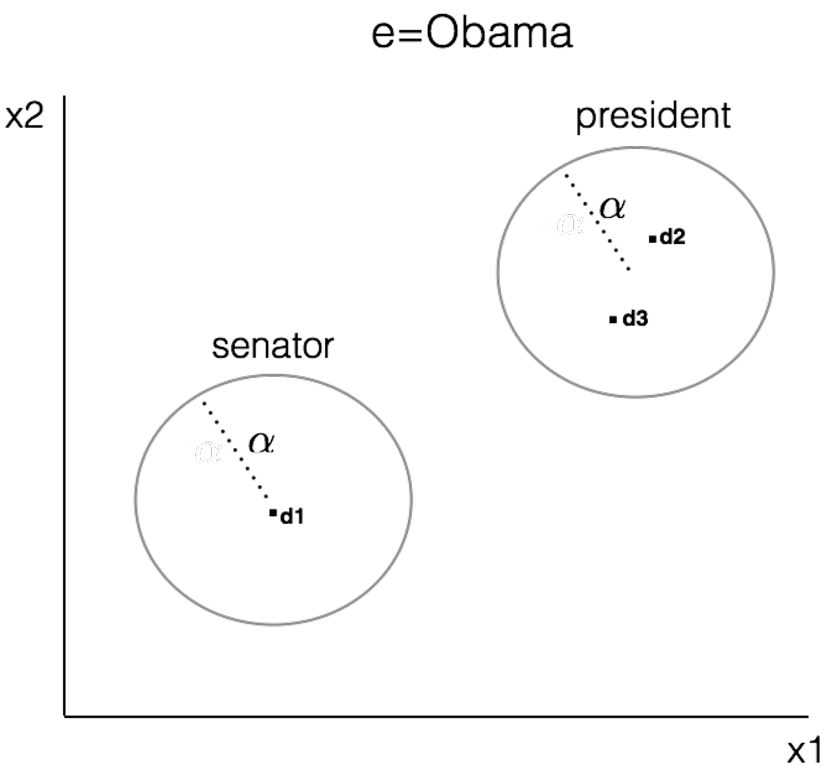
\includegraphics[width=0.7\columnwidth]{fig/obamaExample.pdf}
\caption{Example of Non-parametric Clustering}
\label{obama}
\end{figure}

Figure \ref{obama} illustrates an example of such clustering, using two-dimensions to represent the vectors.
Let's assume document $d_1$ appears in the stream first, and mentions the days Barack Obama was a senator. As it is the first document referring to the entity Obama, we add a new topic cluster $senator$ with vector $v_{d_1}$. 
Then, document $d_2$ appears in the stream, and refers to Obama as being elected President of the United States.
The distance with the previous cluster $senator$ is greater than $\alpha$ due to semantic difference in the words, therefore the algorithm proceeds to create a new topic cluster $president$ centered at $v_{d_2}$. 
Finally, $d_3$ enters the stream. 
It talks about Obama as the current President of the U.S. 
The algorithm compares its distance to the previous clusters and finds that it is closest to the $president$ cluster. 
The distance is less than $\alpha$, hence it adds $d_3$ to the $president$ cluster and updates the cluster center. 

\subsection{Staleness}
\label{staleness}

% problem
We have been concerned with detecting whether a document $d$ contains a novel context in terms of the documents seen so far.
By representing the context of an entity as a set of topic clusters, each with an embedding vector, we are able to accurately summarize the entity's context information. We expect that documents that are not close to existing clusters contain novel information.
Unfortunately, this representation ignores the timeliness of the information, and it is quite possible that a document that is similar to existing clusters contains novel information.
For example, when a document describes Obama victory in an election, it may be assigned to an existing cluster describing a previous election he won, nonetheless it actually contains new information.

% solution
A potential solution is to keep track of when the last document was assigned to a cluster, however, KBA challenge requires \emph{all} documents that contain novel information within a time frame to be marked vital as per the timeliness of the document.
Such timeliness is a subjective interpretation that can vary per entity and event. 
As an example let's assume that several documents talk about an event that happened to entity $e$. 
During a ``short'' time frame (here is where the subjective interpretation comes in) that information can be considered new. 
After a while, that new information transitions to a background state, so as the documents transition from being \emph{vital} to \emph{non-vital}.

%As mentioned in section \ref{background}, the notion of $vitalness$ is closely related to the timeliness of the new information. 

In order to address such temporal dynamics that capture novelty and transition documents from a \emph{vital} to a \emph{non-vital} state, we propose a dynamic staleness measure $\lambda_i$, $0 < \lambda_i \leq 1$. 
This staleness measure can be used both for entities and topic clusters.
Low staleness of the assigned entity/cluster represents \emph{vital} documents, while high staleness intends to represent \emph{non-vital} ones.

The staleness of an entity/cluster at any time $t$ depends on the staleness and the time of the last document $d_j$ assigned to the entity/cluster. % when a relevant document is observed is a two-step process, an exponential decrease followed by a constant increase. $t_{i-1}$ is the $i-1$ document timestamp, 
The staleness decay rate is exponential, and is controlled by the hyperparameter $\gamma_{dec}$:
\begin{equation}
\label{decrease}
\lambda_t = \lambda_{j} \exp{(-\gamma_{dec} \frac{t-t_j}{T})}
\end{equation}
where $\gamma_{dec} \geq 0$, $t_j$ and $\lambda_j$ are the timestamp and staleness of the last document assigned to the entity/cluster, and $T$ is a constant (used to transform the units of time). %, and $\lambda^{inc}_{i-1}$ is the staleness increase (defined below) at a previous timestamp.

When a new document $d_i$ is assigned to an entity/cluster at time $t_i$, we can estimate the staleness of the entity/cluster at that time using the above equation, $\lambda_{t_i} = \lambda_{i-1} \exp{(-\gamma_{dec} \frac{t_i-t_{i-1}}{T})}$.
This staleness can be used to estimate the novelty of the information in $d_i$, i.e. a low $\lambda_{t_i}$ suggests the document contains information that has not been observed for a while.

Thereafter, since we have just observed a relevant document for the entity/cluster, we need to increase its staleness. 
%In case we use staleness as an entity's measure, $\lambda^{inc}_{i-1}$ alludes to the staleness of the previous document in the stream that refers to the same entity as document $i$.
%If we use staleness as a topic cluster's measure, $\lambda^{inc}_{i-1}$ refers to the staleness of the previous document that belongs to the same topic cluster as document $i$.
We use a simple interpolation to increase it, using $\gamma_{inc}$ to control the change as follows:
\begin{equation}
\lambda_i = 1 - \gamma_{inc}(1 - \lambda_{t_i})
\end{equation}
where $0 \leq \gamma_{inc} \leq 1$.
The staleness for the entity/cluster is now $\lambda_i$, which is used when the next document $d_{i+1}$ is observed.

%\subsubsection{Examples}
\begin{figure}[tb]
\centering
% use the png to remove the lambdaInc and decrease from the figures
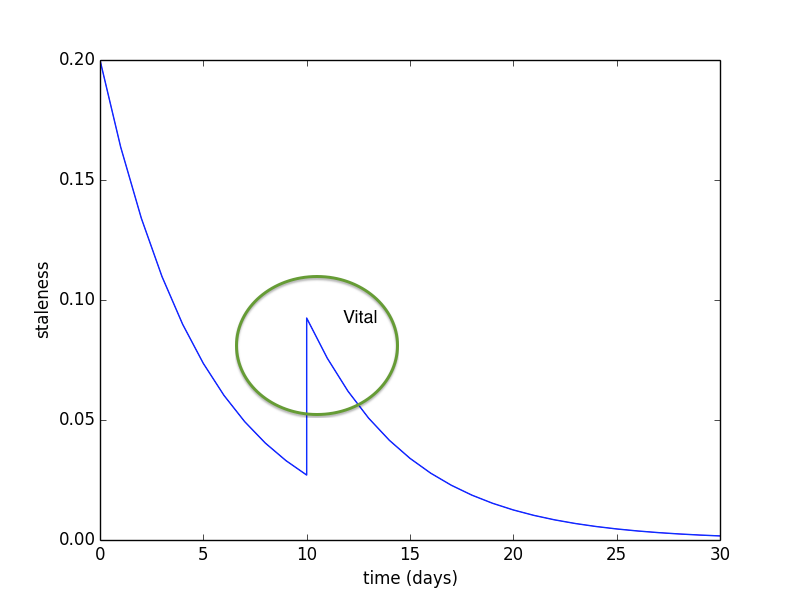
\includegraphics[width=0.7\columnwidth]{fig/staleness1.png}
\caption{Staleness of Unpopular Entity}
\label{stalenesslow}
\end{figure}

%Figures \ref{stalenesslow} and \ref{stalenessmedium} illustrate some toy examples to further understand the intuition behind staleness.
Figure \ref{stalenesslow} illustrates an example of an entity with a decreasing staleness. 
There are almost no documents referring to the entity. 
As soon as some activity is detected, i.e. a document mentioning the entity appears ($t=10$), the staleness increases slightly. 
Given the fact that there's not much information about the entity, every new document would drive an update to the entity's profile, strongly suggesting vitalness.

Figure \ref{stalenessmedium} aims to represent staleness of an entity with fluctuating activity levels in the stream of documents. At time $t\mathord{=}10$, a main event involving the entity starts and continues for a long period of time, showing a growing trend in popularity. 
At the beginning, those documents can be considered vital, but as time goes by and documents continue commenting on the same event, the information starts staling, clearly indicating non-vitalness.
Near $t\mathord{=}40$, the event can be considered over, a steep decrease in popularity is shown. At a later time, $t=50$, a new event occurs, which denotes vitalness.

\begin{figure}[tb]
\centering
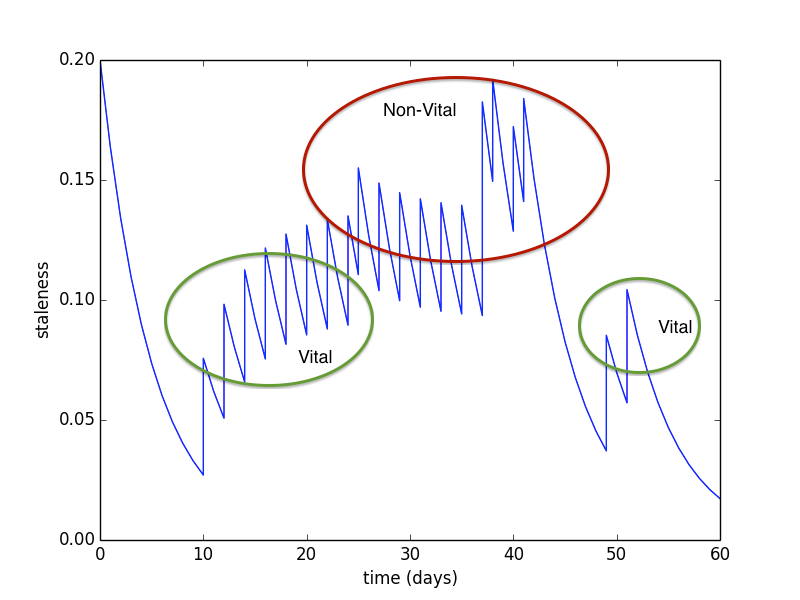
\includegraphics[width=0.7\columnwidth]{fig/staleness2.png}
\caption{Staleness of Entity with Fluctuating Popularity}
\label{stalenessmedium}
\end{figure}

\section{Visualization for Accelerate and Create}

%There is an urgent need for efficient analysis of constantly increasing text collections.
Intuitive and effective visualization techniques can provide valuable tools in assisting editors to populate entity profiles and to perform exploratory analysis of large collections of documents. 
In this section, we describe the requirements of such visualization tools for streaming documents.
Then, we present our prototype data visualization software for the Accelerate and Create task, that enables users to enlarge certain parts of the visual space while simultaneously shrinking the context, a technique called focus-plus-context~\cite{Artur2010}.

\subsection{Goals and Challenges}

Visual exploration of text streams is a challenging task. As text streams continuously evolve, visualization methods should allow tracing the temporal evolution of existing topics, detection of new ones, and examination of the relationships between them.
Such systems should also allow users to interactively change the information they are seeking at any time. 
Interactivity is therefore a crucial factor in a domain where users do not know the text documents in advance \cite{AlsakranCLZYDL12}.

In this work we intend to provide an easy-to-use vizualization that enables users debug what is going on in the sytem. We provide different mechanisms to select data based on users interests; in particular we focus our attention on providing interactive time-series widgets.

\begin{figure}[tb]
        \centering
        \begin{subfigure}[b]{0.4\textwidth}
			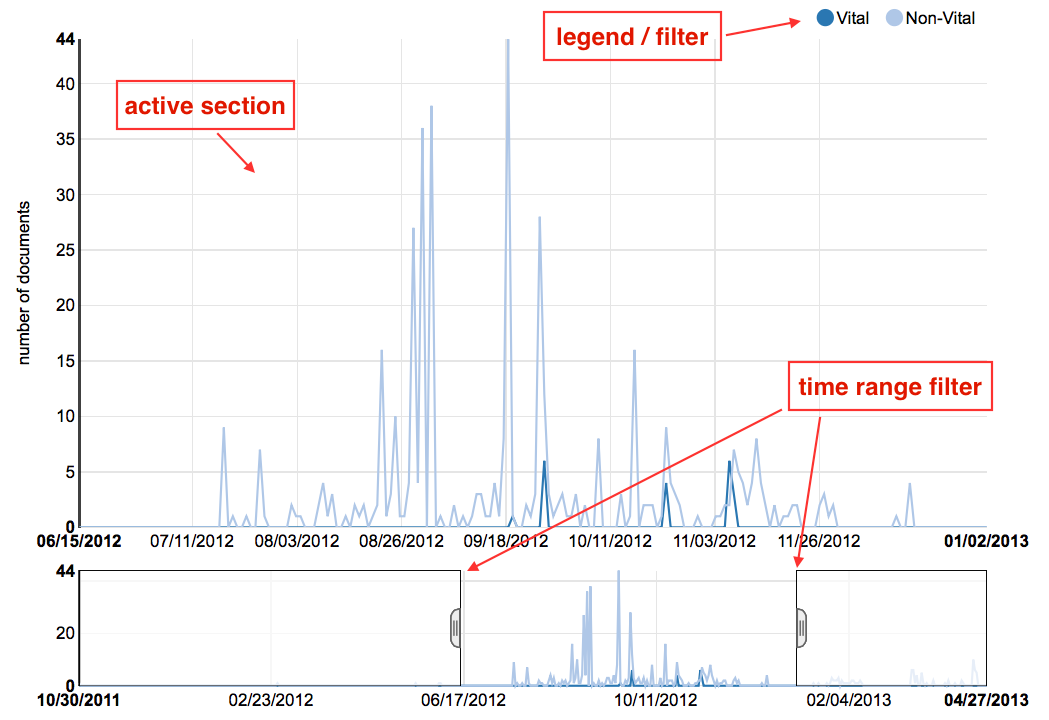
\includegraphics[width=\textwidth]{fig/vitalDistribution.png}
			\caption{Predictions Distribution chart example}
			\label{vitalEvol}
        \end{subfigure}
        \\
        \begin{subfigure}[b]{0.4\textwidth}
            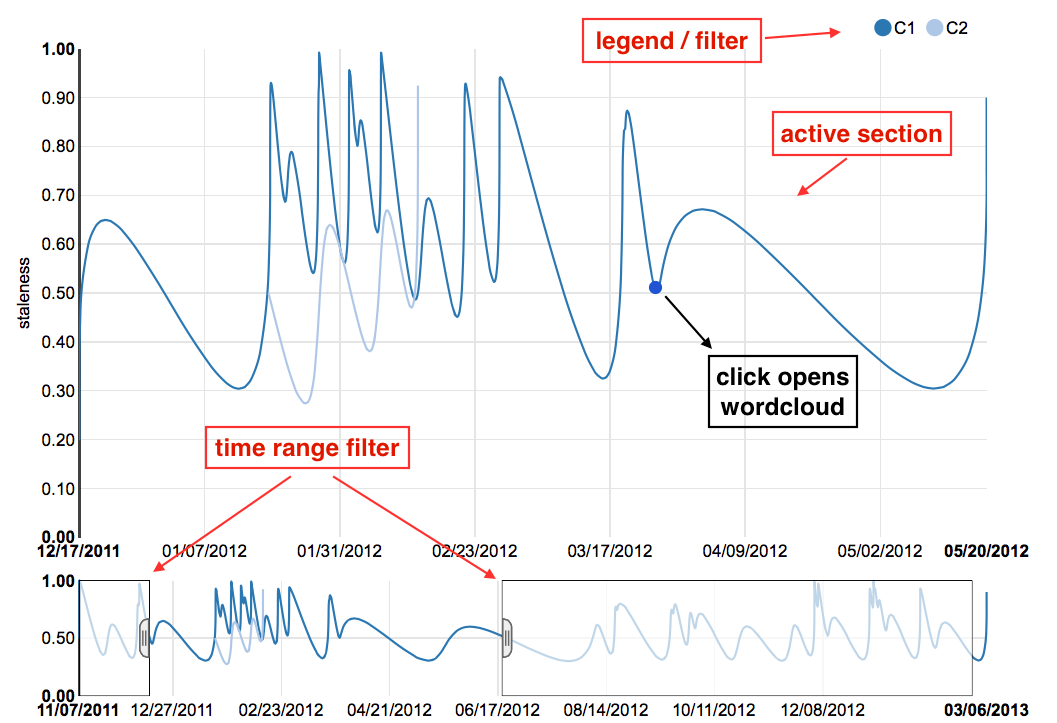
\includegraphics[width=\textwidth]{fig/stalenessDistribution.png}
			\caption{Staleness chart example}
			\label{stalenessEvol}
        \end{subfigure}
        \\
        \begin{subfigure}[b]{0.25\textwidth}
    		\raisebox{0mm}{\includegraphics[width=\textwidth]{fig/wordclouds.png}}
			\caption{Topic cluster example}
			\label{wordcloud}
        \end{subfigure}
        \caption{Staleness and Topic cluster evolution}
\end{figure}

\subsection{Our Implementation}

We propose a browser-based visualization prototype that enables users to switch between multiple entities of interest, select the time ranges to explore over, explore the prominence of topics over time, and understand the topics using lists of similar words.

%\begin{figure}[tb]
%\centering
%\end{figure}

The visualization tool initiates with the user selecting an entity of interest using an autocomplete-enabled text-box.
For the selected entity, our visualization consists of two views: \emph{Document} and \emph{Topic}.

The \emph{Document} view shows the distribution of vital and non-vital documents over the whole timeline, summarizing and differentiating the time frames when the documents simply refer to the entity, and when they contain vital information.
Figure \ref{vitalEvol} illustrates the distribution of predictions of entity \emph{Kshama Sawant} in a specific period of time. %The entity search box has been omitted for space reasons.
Once the interesting time frames have been identified, this view also allows the user to navigate to and read individual documents. 

The \emph{Topic} view shows the evolution of the topic clusters for the entity, illustrating the predicted proportion of topic clusters over time.
This view primarily plots the staleness of a cluster over time, indicating when a cluster was started, mentioned in the documents, and fall into obsolescence. 
The user can also study the topics in finer detail, clicking on any point in the timeline brings up a word cloud representation of the topic at that time.
Figure \ref{stalenessEvol} shows the staleness evolution for the different topic clusters of entity \emph{Mike Kluse}. 
%The user can select any point in the line to further inspect the topic cluster. 
Figure \ref{wordcloud} is the result of a user's click on the point highlighted in Figure \ref{stalenessEvol}. 
It shows the closest words to the topic cluster C1 at that time.

Both views consist of a timeline over the whole stream, allowing users to quickly navigate them over different time frames.
The timeline is an active (zoomed) section which can be changed using the time range filters located below. Legends can also act as filters, users have the possibility to observe particular clusters or predictions by selecting them in the legend region.
These interactive time-series controls combined with the word cloud representations allow users to explore streaming data and filter information based on their needs.

\section{Related Work}
\label{related}

Several knowledge based acceleration competitions have been done in the recent past, testifying the great progress achieved in these fields~\cite{gross_doucet_toivonen_trec12}. 
\citet{xitong12} present one of the best performing systems in TREC KBA 2012. 
They created broader representations of entities' profiles based on a Wikipedia snapshot and considered the anchor text of all internal Wikipedia links as related entities. In TREC KBA 2013 competition, different families of methods were proposed, including query expansion, classification, and learning to rank. 

Our strategy is somewhat similar to \citet{jingang13} in the sense that we first target a high recall system and then apply different classification methods to differentiate between \emph{vital} and \emph{non-vital} documents. 
One key difference is that we do not exploit any external resources to construct features, e.g. we do not use Wikipedia entity pages nor existing citations in the Wikipedia page of an entity. 

Representing words as continuous vectors has been around for a while~\cite{Hinton87, Elman90findingstructure}. 
The progress of machine learning techniques in recent years enabled training more complex models on much larger data sets \cite{mikolovChen}. 
One popular approach to increase accuracy in existing system is to use unsupervised methods to create word features, or to download word features that have already been produced \cite{Turian10wordrepresentations}. In our method, we do the latter, we use already induced word embedding features in order to improve its accuracy. To our best knowledge, no techniques propose using distributed word embeddings representations for solving the vital filtering problem.

One pioneering work on detecting novel documents was introduced by \citet{Zhang2002}. In their work, they explicitly model relevance and redundancy as separate concepts. They propose different redundancy measures and empirically show that the cosine similarity metric is effective in identifying redundant documents; one limitation is that they just keep the 10 most recent documents for a profile. In our method, we can keep the whole history of documents for a given entity, which allows a more accurate estimate of the query document's redundancy.

Since then, many work has been made on scaling novel detection algorithms, also known as First Story Detection, in streaming settings, by either using LSH \cite{Petrovic2010} or just using simple heuristics \cite{Luo2007}. While their work mainly focuses on making the computation tractable, our work focuses more on achieving high accuracy. 

Another example that addresses the problem of staleness detection was done by \citet{gamon}, where he builds an association graph connecting sentences and sentence fragments, and uses graph-based features as good indicators of lack of novelty. Though the task is somewhat similar, is more limited in the sense that they do not need to model the transition from new to background information where, in principle, all documents are citation worthy.

Streaming document filtering is also related to several other fields, including but not limited to, entity linking \cite{KBP11}, text categorization \cite{HLTCOE12}, news surveillance \cite{Steinberger14}, and cross-document coreference~\cite{RaoMD10,singh11:acl}.


\section{KBA Vital Filtering Evaluation}
\label{evaluation}

\subsection{Data}
\label{data}

To assess our method we use TREC KBA 2014 filtered stream corpus. It has around 20M documents annotated with BBN's Serif NLP tools, including within-doc coreference and dependency parse trees. Further, we use the 71 target entities given by KBA organizers for the Vital Filtering task. Among the 20M documents, around 28K have truth labels. From these, only 8K are training instances while the rest are test examples.
%\subsubsection{Preprocess}
We preprocess the corpus to filter the documents that contain exact string matches to the target entities names, including canonical and surface form names.

\subsection{Features}
\label{feat}

Our approach extends the classifier introduced by \citet{jingang13}.
We construct a basic set of features based on the document and the entity of interest.
Using our representation, we include additional features for the embedding, clustering, and staleness.
A summary of the features we use is presented in Table \ref{features}. 

%\comment{

\begin{table}[tb]
\center
{\small
\begin{tabular}{p{0.2\columnwidth}p{0.73\columnwidth}}
\toprule
%\textbf{FEATURE} & \textbf{DESCRIPTION} \\ 
\multicolumn{2}{c}{\textbf{Basic Features, $F_b$}} \\ %\hline
\midrule
\multicolumn{2}{l}{\emph{Based on document $d$}} \\ %\hline
$\log(len(d))$ & log of the length of $d$ \\ %\hline
$source(d)$ & discretized source of $d$ \\
\multicolumn{2}{l}{\emph{Based on document $d$ and target entity $e$}} \\ %\hline
$n(d,e)$ & \# of occurrences of target entity $e$ in $d$ \\
$n(d,e^p)$ & \# of occurrences of partial name of $e$ in $d$ \\
$\text{fpos}(d,e)$ & position of first occurrence of entity $e$ in $d$ \\
$\text{fpos}_n(d,e)$ & $\text{fpos}(d,e)$ normalized by document length \\
$\text{fpos}(d,e^p)$ & position of first partial occurrence of $e$ in $d$ \\
$\text{fpos}_n(d,e^p)$ & $\text{fpos}(d,e_p)$ normalized by document length \\
$\text{lpos}(d,e)$ & position of last occurrence of entity $e$ in $d$ \\
$\text{lpos}_n(d,e)$ & $\text{lpos}(d,e)$ normalized by document length \\
$\text{lpos}(d,e^p)$ & position of last partial occurrence of entity $e$ in $d$ \\
$\text{lpos}_n(d,e^p)$ & $\text{lpos}(d,e^p)$ normalized by document length \\ 
$\text{spread}(d,e)$ & $\text{lpos}(d,e) - \text{fpos}(d,e)$ \\
$\text{spread}_n(d,e)$ & $\text{spread}(d,e)$ normalized by document length \\
$\text{spread}(d,e^p)$ & $\text{lpos}(d,e^p)\mathord{-}\text{fpos}(d,e^p)$ \\
$\text{spread}_n(d,e^p)$ & $\text{spread}(d,e^p)$ normalized by document length \\ 
\midrule
\multicolumn{2}{c}{\textbf{Embedding Features, $F_e$}} \\ %\hline
\midrule
\multicolumn{2}{l}{\emph{Based on combined embedding, $F_e^c$}} \\ %\hline
  $v_d$ & mean word embedding representation of $d$ \\
  $\text{zero}(v_d)$& $\mathbbm{1}_{v_d=0}$, set to 1 if $v_d$ is $0$ \\
\multicolumn{2}{l}{\emph{Based on POS embeddings, $F_e^p$}} \\ %\hline 
  $v_{d_n}$ & mean word embedding representation of nouns in $d$ \\
  $\text{zero}(v_{d_n})$& $\mathbbm{1}_{v_{d_n}=0}$, set to 1 if $v_{d_n}$ is $0$ \\
  $v_{d_v}$ & mean word embedding representation of verbs in $d$ \\
  $\text{zero}(v_{d_v})$& $\mathbbm{1}_{v_{d_v}=0}$, set to 1 if $v_{d_v}$ is $0$ \\
  %$v_{d_{pn}}$ & mean word embedding representation of proper nouns in $d$ \\
  %$\text{zero}(v_{d_{pn}})$& $\mathbbm{1}_{v_{d_{pn}}=0}$, set to 1 if $v_{d_{pn}}$ is $0$ \\
\midrule
\multicolumn{2}{c}{\textbf{Clustering Features, $F_c$}} \\ %\hline
\midrule
  $\min_c(v_d,v_c)$& minimum distance of $v_d$ to topic clusters of $e$ \\
  $\text{avg}_c(v_d,v_c)$& average distance of $v_d$ to topic clusters of $e$ \\
\midrule
\multicolumn{2}{c}{\textbf{Temporal Features, $F_t$}} \\ %\hline
\midrule
  $\lambda(e)$& current staleness of entity $e$ \\
  $\lambda(e,c)$& current staleness of topic $c$ of target entity $e$ \\
\bottomrule
\end{tabular}
} % end of small
\caption{Features for Vital Filtering classification}
\label{features}
\end{table}

%} %end comment

\subsection{Relevance Classification}

%\subsubsection{Categories}
%\label{subcat}
TREC KBA 2014 corpus contain documents that do not refer to the target entities, even though they may contain mentions to them. We therefore need to use a \emph{non-referent} category of documents. 
%
A \emph{non-referent} document denotes that it does not refer to a target entity or the context is so ambiguous that it is impossible to decide whether the mention refers to an entity or not. An example of the former case is ``Barack Ferrazzano provides a wide range of business-oriented legal''. It clearly does not refer to Barack Obama. For the latter, an example is ``Barack is a great father and a better husband''. The mention ``Barack'' may refer to any married parent named Barack, therefore, we consider it \emph{non-referent}.
%
The \emph{vital} and \emph{non-vital} classes described in section \ref{background} fall into a \emph{referent} (or \emph{relevant}) category, which contains documents that refer to the target entities.

Due to the fact that not all documents in the corpus refer to the target entities, we include an extra step in our classification process, as shown in Figure \ref{classifier}. We introduce an additional classifier, called $rnr$, which is trained offline and classifies documents as \emph{referent} or \emph{non-referent}.
Consequently, in every experiment, each document goes first through the \emph{rnr} classifier. Only the \emph{referent} documents outputted by \emph{rnr} are used as inputs to the \emph{vnv} classifier, which discriminates between \emph{vital} and \emph{non-vital} documents, the overall focus of this work.

\begin{figure}[tb]
\centering
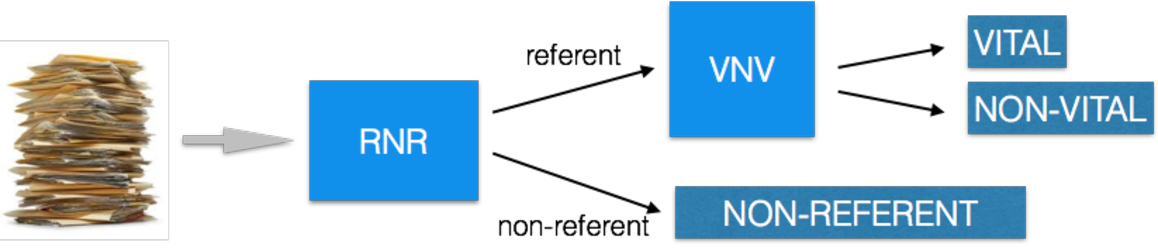
\includegraphics[width=1\columnwidth]{fig/classifier.pdf}
\caption{Classification process}
\label{classifier}
\end{figure}


\subsection{Methods}
\label{expe}

We use randomized tree ensembles classifiers \cite{GEW06a} for both \emph{rnr} and \emph{vnv}, each composed of $100$ weak learners. Each tree in the ensembles has a maximum depth of $150$.
%
All the experiments use the same \emph{rnr} model trained with the basic features listed in section \ref{feat}.
The different methods differ on the features used to train and test the \emph{vnv} classifier.

\begin{itemize}
  \item {\textit{Baseline Single}}: baseline method that uses $F_b$ features. \citet{jingang13, bellogin13} have a similar method, though they train their models with more features.
  \item {\textit{Baseline Multi-task}}: baseline method similar to {\textit{Baseline Single}} but includes multi-task learning \cite{Caruana93multitasklearning}.
  \item {\textit{Embedding Combined}}: similar to {\textit{Baseline Multi-task}} but includes $F_e^c$ features. The word embeddings are computed using the Google News dataset. Each document has a single combined embedding, which is calculated from the nouns and verbs found in the linguistic context of the entities' mentions, as described in section \ref{docwordemb}.
  \item {\textit{Embedding POS}}: similar to {\textit{Embedding Combined}} but uses $F_e^p$ features. Instead of a single combined embedding per document, it has one embedding per word type in each document, i.e. it computes separate embeddings for nouns and verbs. %It uses the part of speech annotations in the documents to easily extract the different word types.
  \item {\textit{Mean Dynamic}}: similar to the {\textit{Embedding POS}} method but it includes the $F_t$ features.
  \item {\textit{Clustering Static}}: similar to the {\textit{Embedding POS}} method but it includes the $F_c$ features.
  \item {\textit{Clustering Dynamic}}: similar to the {\textit{Embedding POS}} method but it includes $F_t$ and $F_c$ features.
\end{itemize}


%Official
\begin{table*}[tb]
{\small
\begin{center}
\begin{tabular}{llccccccccc} 
\toprule
  \multirow{2}{*}{\textbf{Model}} & 
  \multirow{2}{*}{\textbf{Features}} & 
  \multicolumn{3}{c}{\textbf{Vital only}, \emph{micro}} &
  \multicolumn{3}{c}{\textbf{Vital only}, \emph{macro}}
\\ 
  \cmidrule(lr){3-5}
  \cmidrule(lr){6-8}
&   & 
  \textbf{P} & \textbf{R} & \textbf{F1} & 
  \textbf{P} & \textbf{R} & \textbf{F1} \\ 
\midrule
{\textit{Baseline Single}} & $F_b$ &
	53.9  \hspace{1mm} 26.6 & 26.5 \hspace{1mm} 63.4 & 35.5 \hspace{1mm} 37.5 &
  47.5  \hspace{1mm} 36.6 & 23.8 \hspace{1mm} 94.0 & 31.7 \hspace{1mm} 52.7 \\
{\textit{Baseline Multi-task}} & $F_b$ &
  60.7 \hspace{1mm} 60.7 & 41.4 \hspace{1mm} 41.4 & 49.2 \hspace{1mm} 49.2 &
  36.7 \hspace{1mm} 36.6 & 40.5 \hspace{1mm} 94.0 & 38.5 \hspace{1mm} 52.7 \\
{\textit{Embedding Combined}} & $F_b+F_e^c$ & 
  54.7 \hspace{1mm} 54.7 & 52.1 \hspace{1mm} 51.8 & 53.4 \hspace{1mm} 53.2 &
  44.9 \hspace{1mm} 38.3 & 37.6 \hspace{1mm} 85.5 & 40.9 \hspace{1mm} 52.9 \\
{\textit{Embedding POS}} & $F_b+F_e^p$ & 
  53.9 \hspace{1mm} 49.9 & 46.4 \hspace{1mm} 53.1 & 49.8 \hspace{1mm} 51.4 &
  44.0 \hspace{1mm} 36.6 & 32.9 \hspace{1mm} 94.0 & 37.6 \hspace{1mm} 52.7 \\
{\textit{Mean Dynamic}} & $F_b+F_e^p+F_t$ & 
  57.3 \hspace{1mm} 57.3 & 48.3 \hspace{1mm} 48.3 & 52.4 \hspace{1mm} 52.4 &
  47.5 \hspace{1mm} 39.1 & 33.8 \hspace{1mm} 85.8 & 39.5 \hspace{1mm} 53.7 \\
{\textit{Clustering Static}} & $F_b+F_e^p+F_c$ & 
	57.0 \hspace{1mm} 57.0 & 49.0 \hspace{1mm} 48.9 & 52.7 \hspace{1mm} 52.6 &
	46.4 \hspace{1mm} 38.7 & 34.2 \hspace{1mm} 85.0 & 39.4 \hspace{1mm} 53.2 \\
{\textit{Clustering Dynamic}} & $F_b+F_e^p+F_c+F_t$ &
  56.2 \hspace{1mm} 56.2 & 48.1 \hspace{1mm} 48.1 & 51.8 \hspace{1mm} 51.8 &
	46.1 \hspace{1mm} 36.6 & 32.6 \hspace{1mm} 94.0 & 38.2 \hspace{1mm} 52.7 \\
 
\bottomrule
\end{tabular}
\end{center}
}
\caption{UW Vital Filtering official and revised percentage results for TREC KBA 2014}
\label{officialRes}
\end{table*}


%Official
%\begin{table*}[tb]
%{\small
%\begin{center}
%\begin{tabular}{llccccccccc} 
%\toprule
%  \multirow{2}{*}{\textbf{Model}} & 
%  \multirow{2}{*}{\textbf{Features}} & 
%  \multicolumn{3}{c}{\textbf{Vital only}, \emph{micro}} &
%  \multicolumn{3}{c}{\textbf{Vital only}, \emph{macro}}
%\\ 
%  \cmidrule(lr){3-5}
%  \cmidrule(lr){6-8}
%&   & 
%  \textbf{P} & \textbf{R} & \textbf{F1} & 
%  \textbf{P} & \textbf{R} & \textbf{F1} \\ 
%\midrule
%{\textit{Baseline Single}} & $F_b$ &
%  53.9  & 26.5 & 35.5 &
%  47.5  & 23.8 & 31.7 \\
%{\textit{Baseline Multi-task}} & $F_b$ &
%  60.7 & 41.4 & 49.2 &
%  36.7 & 40.5 & 38.5 \\
%{\textit{Embedding Combined}} & $F_b+F_e^c$ & 
%  54.7 & 52.1 & 53.4 &
%  44.9 & 37.6 & 40.9 \\
%{\textit{Embedding POS}} & $F_b+F_e^p$ & 
%  53.9 & 46.4 & 49.8 &
%  44.0 & 32.9 & 37.6 \\
%{\textit{Mean Dynamic}} & $F_b+F_e^p+F_t$ & 
%  57.3 & 48.3 & 52.4 &
%  47.5 & 33.8 & 39.5 \\
%{\textit{Clustering Static}} & $F_b+F_e^p+F_c$ & 
%  57.0 & 49.0 & 52.7 &
%  46.4 & 34.2 & 39.4 \\
%{\textit{Clustering Dynamic}} & $F_b+F_e^p+F_c+F_t$ &
%  56.2 & 48.1 & 51.8 &
%  46.1 & 32.6 & 38.2 \\
%\bottomrule
%\end{tabular}
%\end{center}
%}
%\caption{UW Vital Filtering official percentage results for TREC KBA 2014}
%\label{officialRes}
%\end{table*}



% Revised
%\begin{table*}[tb]
%{\small
%\begin{center}
%\begin{tabular}{llccccccccc} 
%\toprule
%  \multirow{3}{*}{\textbf{Model}} & 
%  \multirow{3}{*}{\textbf{Features}} & 
%  \multicolumn{3}{c}{\textbf{Vital only}, \emph{micro}} &
%  \multicolumn{3}{c}{\textbf{Vital only}, \emph{macro}}
%\\ 
%  \cmidrule(lr){3-5}
%  \cmidrule(lr){6-8}
%&   & 
%  \textbf{P} & \textbf{R} & \textbf{F1} & 
%  \textbf{P} & \textbf{R} & \textbf{F1} \\ 
%\midrule
%{\textit{Baseline Single}} & $F_b$ &
%  26.6 & 63.4 & 37.5 &
%  36.6 & 94.0 & 52.7 \\
%{\textit{Baseline Multi-task}} & $F_b$ &
%  60.7 & 41.4 & 49.2 &
%  36.6 & 94.0 & 52.7 \\
%{\textit{Embedding Combined}} & $F_b+F_e^c$ & 
%  54.7 & 51.8 & 53.2 &
%  38.3 & 85.5 & 52.9 \\
%{\textit{Embedding POS}} & $F_b+F_e^p$ & 
%  49.9 & 53.1 & 51.4 &
%  36.6 & 94.0 & 52.7 \\
%{\textit{Mean Dynamic}} & $F_b+F_e^p+F_t$ & 
%  57.3 & 48.3 & 52.4 &
%  39.1 & 85.8 & 53.7 \\
%{\textit{Clustering Static}} & $F_b+F_e^p+F_c$ & 
%  57.0 & 48.9 & 52.6 &
%  38.7 & 85.0 & 53.2 \\
%{\textit{Clustering Dynamic}} & $F_b+F_e^p+F_c+F_t$ & 
%  56.2 & 48.1 & 51.8 &
%  36.6 & 94.0 & 52.7 \\
%\bottomrule
%\end{tabular}
%\end{center}
%}
%\caption{UW Vital Filtering revised percentage results for TREC KBA 2014}
%\label{officialRevised}
%\end{table*}


% Unofficial doesn't make sense to include
%\begin{table*}[tb]
%{\small
%\begin{center}
%\begin{tabular}{llccccccccc} 
%\toprule
%  \multirow{3}{*}{\textbf{Model}} & 
%  \multirow{3}{*}{\textbf{Features}} & 
%  \multicolumn{3}{c}{\textbf{Vital only}, \emph{micro}} &
%  \multicolumn{3}{c}{\textbf{Vital only}, \emph{macro}}
%\\ 
%  \cmidrule(lr){3-5}
%  \cmidrule(lr){6-8}
%&   & 
%  \textbf{P} & \textbf{R} & \textbf{F1} & 
%  \textbf{P} & \textbf{R} & \textbf{F1} \\ 
%\midrule
%{\textit{Mean Dynamic}} & $F_b+F_e^c+F_t$ & 
%  52.8 & 51.0 & 51.9 &
%  36.6 & 94.0 & 52.7 \\
%{\textit{Clustering Static}} & $F_b+F_e^c+F_c$ & 
%  52.3 & 52.2 & 52.3 &
%  38.8 & 86.7 & 53.6 \\
%{\textit{Clustering Dynamic}} & $F_b+F_e^c+F_c+F_t$ & 
%  54.9 & 52.1 & 53.4 &
%  38.8 & 86.3 & 53.5 \\
%\bottomrule
%\end{tabular}
%\end{center}
%}
%\caption{UW Vital Filtering unofficial percentage results for TREC KBA 2014}
%\label{unofficial}
%\end{table*}

\section{Results and Discussion}

Table \ref{officialRes} shows the official and revised precision, recall and F1 results of the methods explained in \ref{expe}, computed using KBA scorer tool, using the 2014-07-11 truth data. The \textit{Clustering} models use $\alpha=0.8$. Also, the \textit{Dynamic} methods use $\gamma_{dec}=1$ and $\gamma_{inc}=0.1$.

The official baseline provided by TREC KBA organizers assigns a `vital' rating to every document that matches a surface form name of an entity, assigning a confidence score based on the number of matches of tokens in the name. The values reported by the organizers are: macro-P=0.316, macro-R=0.520, macro-F1=0.393, SU=0.3334 \cite{frank14:overview}.

According to the official results, our system achieved the $2^{nd}$ best precision in the competition, but performed poorly in the overall macro F1 ($8^{th}$ position). Revisiting our submission files, we found that we misinterpreted the concept of confidence. Figure \ref{official:submission} shows that we only make vital predictions with confidence greater than or equal to 500, i.e. the right part of the curve is just constant. We should have also predicted vital with low confidence, i.e. flip our high confidence non-vital predictions to be vital with low confidence. That minor change boosts our recall (in most cases), while the precision slightly suffers, as shown in Figure \ref{official:revised}, leaving our system in the $2^{nd}$ overall position.

{\textit{Baseline Single} performs as expected, i.e. has lower F1 than the other models.
On the other hand, {\textit{Baseline Multi-task}} performs far better that {\textit{Baseline Single} in the official results, which evidences that multi-task learning does work.
Most of the more advanced models perform better than {\textit{Baseline Multi-task}}, both on the official and revised results. Using a combined embedding ({\textit{Embedding Combined}}) outperforms using individual embeddings representations for the different type of words ({\textit{Embedding POS}}).
The staleness and non-parametric clustering runs ({\textit{Mean Dynamic}}, {\textit{Clustering Static}}, {\textit{Clustering Dynamic}}) perform slightly worse than the simple {\textit{Embedding Combined}} method on the official results. Nevertheless, they illustrate the importance of these new features as they use separate embeddings for the different word types, and they all improve the performance of the simple {\textit{Embedding POS}} model. In the revised versions, {\textit{Mean Dynamic}} scores the best F1, followed closely by {\textit{Clustering Static}}, which further evidences the importance of $F_t$ and $F_c$ features.

\def \officialRunWidth {0.23\textwidth}
\begin{figure}[tb]
  \centering
    \begin{subfigure}[b]{\officialRunWidth}
            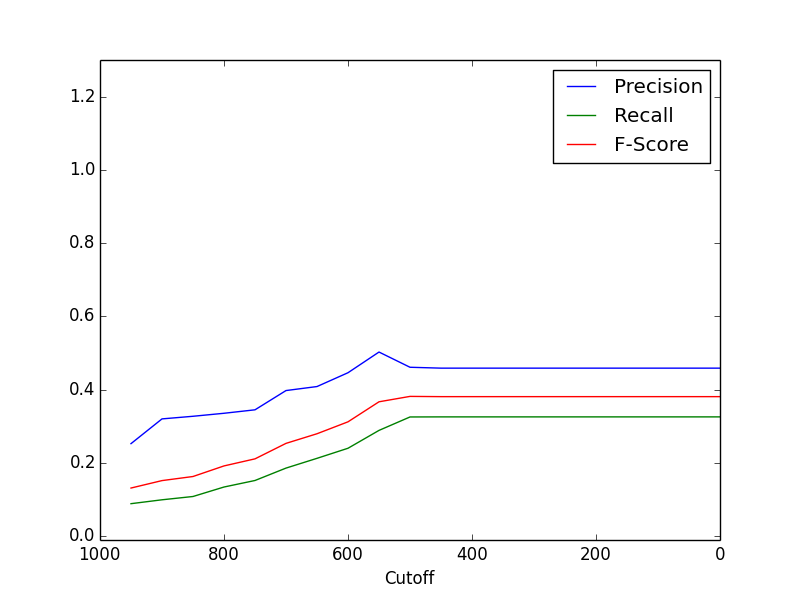
\includegraphics[width=\textwidth]{fig/clust_dyn_wrong.png}
      \caption{Official submission example}
      \label{official:submission}
    \end{subfigure}
    ~
    \begin{subfigure}[b]{\officialRunWidth}
            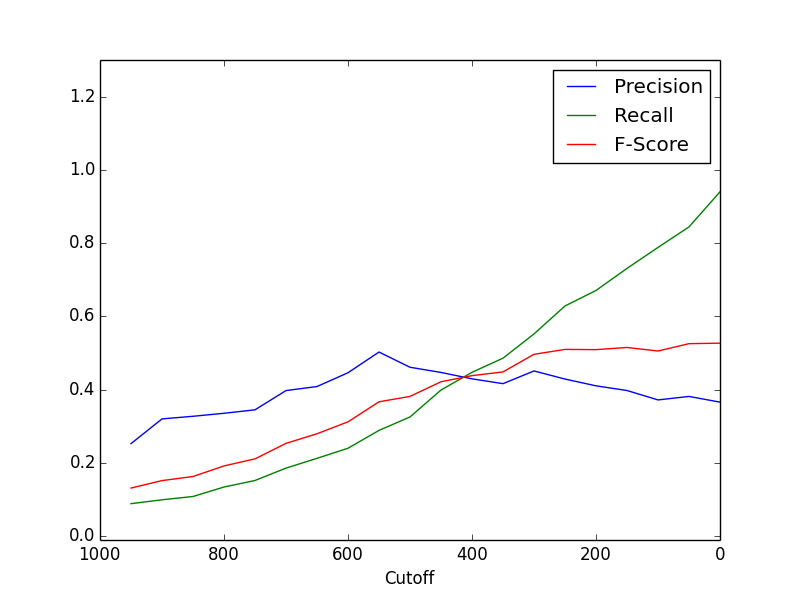
\includegraphics[width=\textwidth]{fig/clust_dyn_right.png}
      \caption{Official submission revised}
      \label{official:revised}
    \end{subfigure}
\caption{P-R-F1 over confidence cutoffs}
\label{submissionAndRevised}
\end{figure}


\def \officialRunWidth {0.23\textwidth}
\begin{figure}[tb]
  \centering
    \begin{subfigure}[b]{\officialRunWidth}
            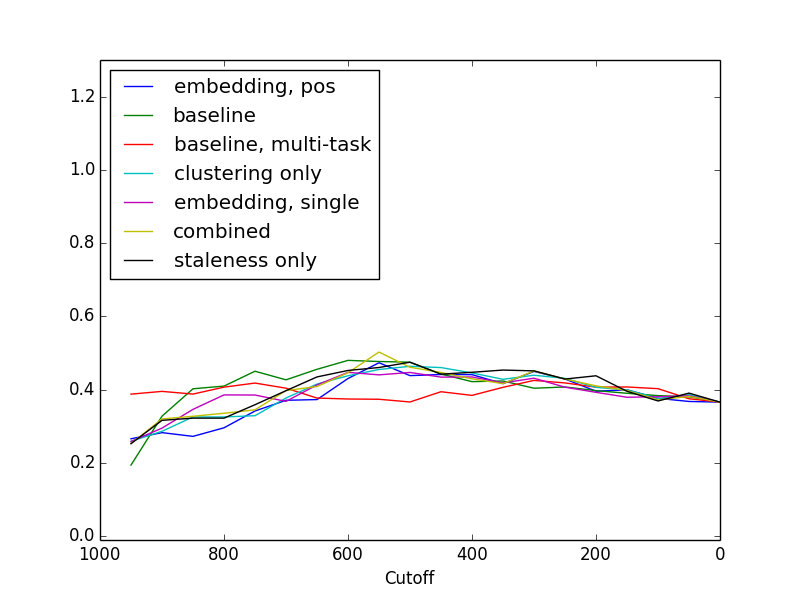
\includegraphics[width=\textwidth]{fig/macroPrecision}
			\caption{Precision}
			\label{official:macroprec}
    \end{subfigure}
    ~
    \begin{subfigure}[b]{\officialRunWidth}
            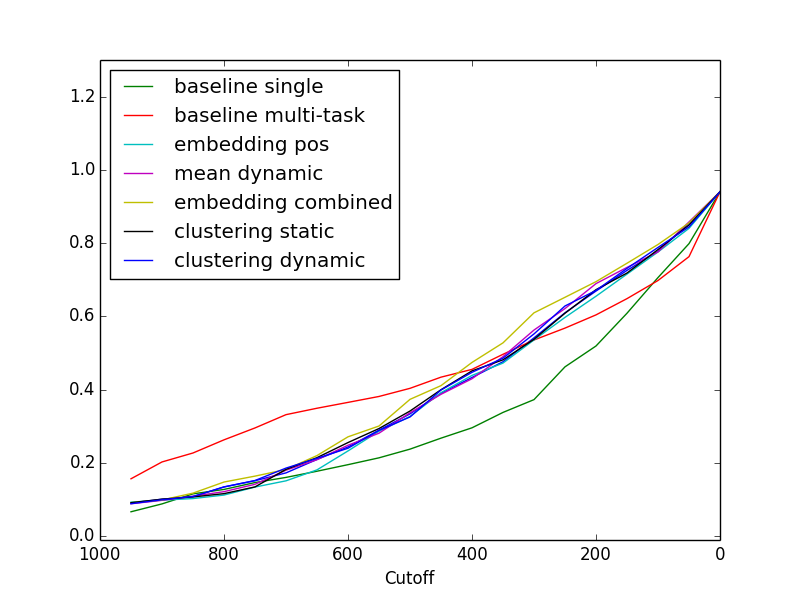
\includegraphics[width=\textwidth]{fig/macroRecall}
			\caption{Recall}
			\label{official:macrorecall}
    \end{subfigure}
    ~
    \begin{subfigure}[b]{\officialRunWidth}
            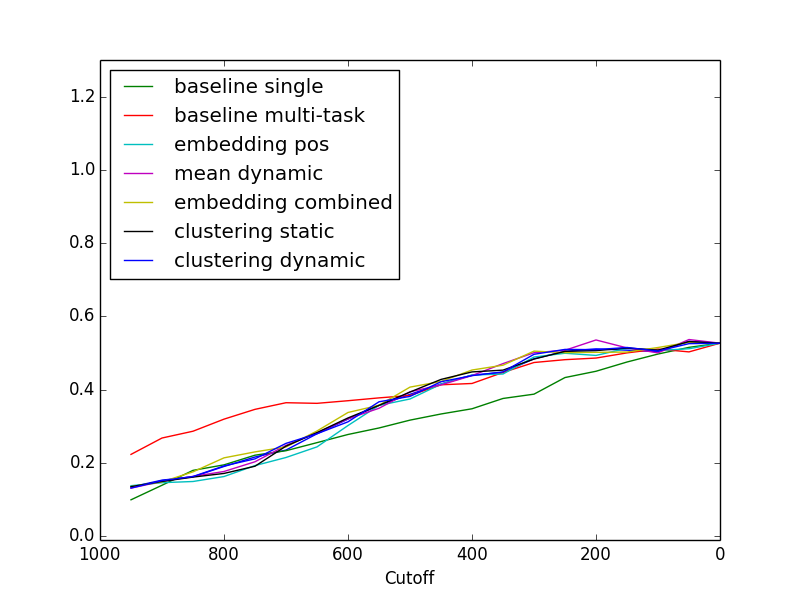
\includegraphics[width=\textwidth]{fig/macroF1}
			\caption{F1}
			\label{official:macrof1}
    \end{subfigure}
    ~
    \begin{subfigure}[b]{\officialRunWidth}
            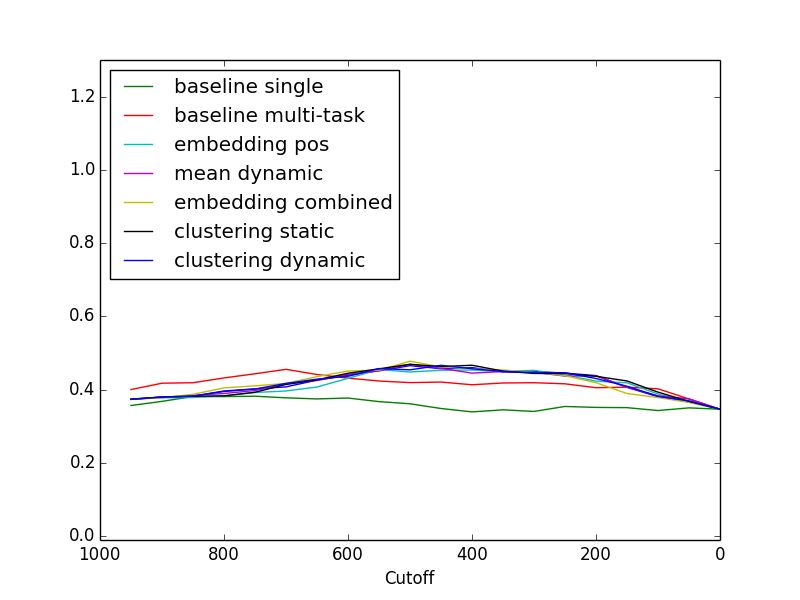
\includegraphics[width=\textwidth]{fig/macroSU}
			\caption{Scaled Utility}
			\label{official:macrosu}
    \end{subfigure}
\caption{Macro P-R-F1-SU over confidence cutoffs}
\label{macroRuns}
\end{figure}

\def \officialRunWidth {0.23\textwidth}
\begin{figure}[tb]
  \centering
    \begin{subfigure}[b]{\officialRunWidth}
            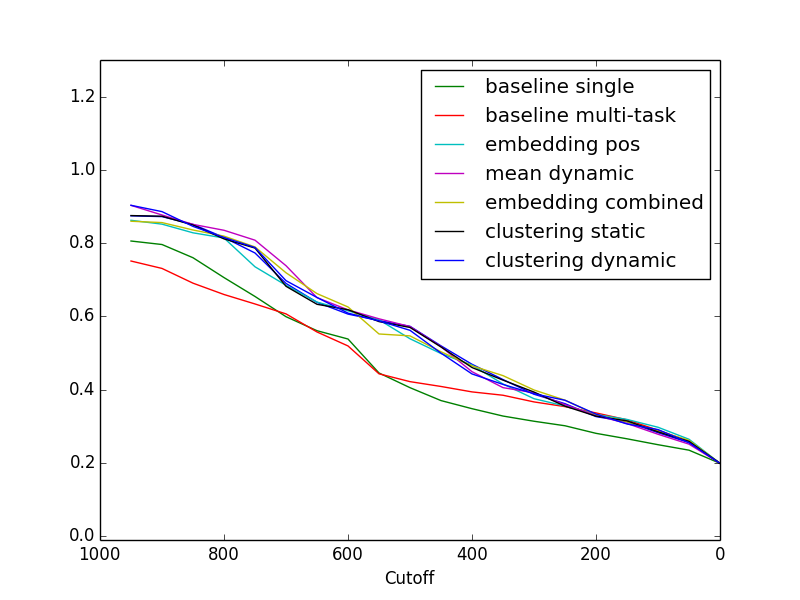
\includegraphics[width=\textwidth]{fig/microPrecision}
      \caption{Precision}
      \label{official:microprec}
    \end{subfigure}
    ~
    \begin{subfigure}[b]{\officialRunWidth}
            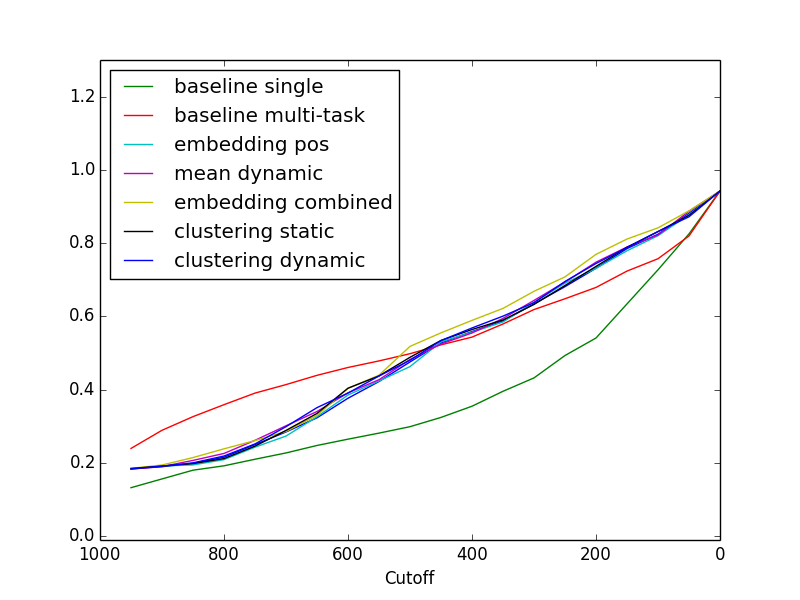
\includegraphics[width=\textwidth]{fig/microRecall}
      \caption{Recall}
      \label{official:microrecall}
    \end{subfigure}
    ~
    \begin{subfigure}[b]{\officialRunWidth}
            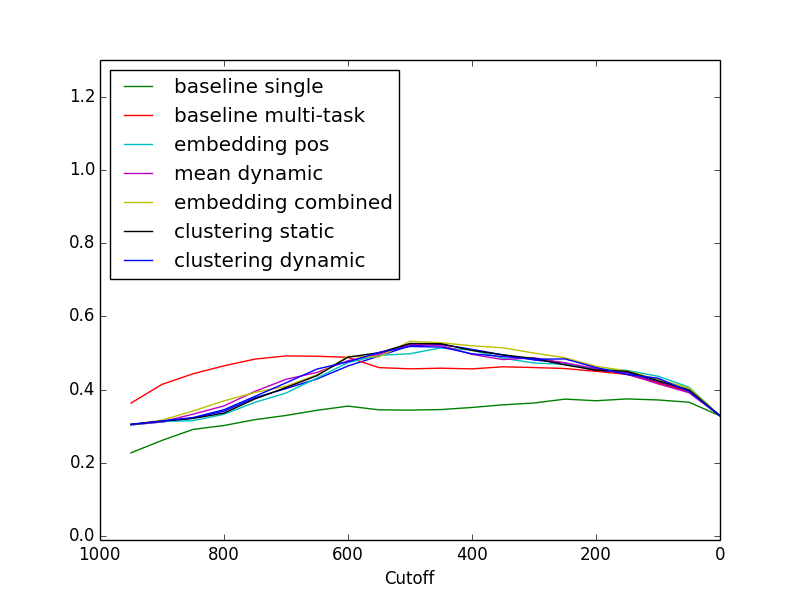
\includegraphics[width=\textwidth]{fig/microF1}
      \caption{F1}
      \label{official:microf1}
    \end{subfigure}
    ~
    \begin{subfigure}[b]{\officialRunWidth}
            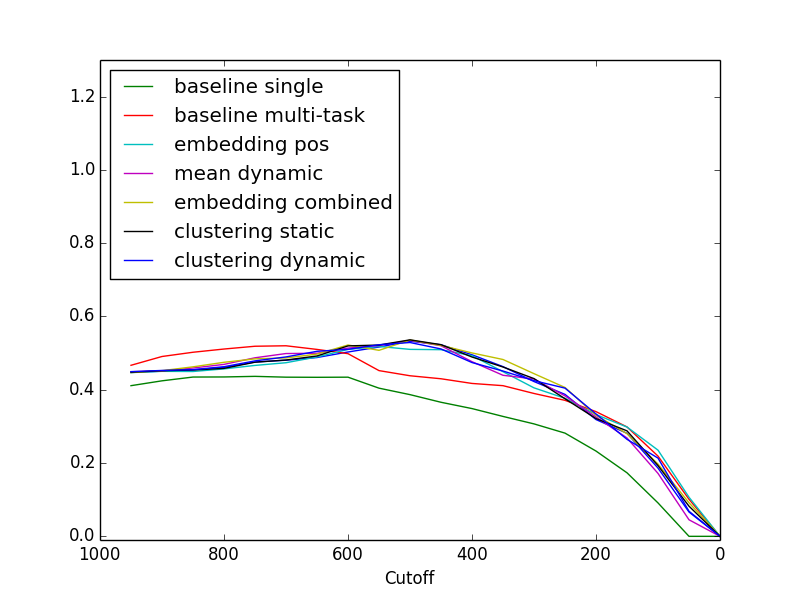
\includegraphics[width=\textwidth]{fig/microSU}
      \caption{Scaled Utility}
      \label{official:microsu}
    \end{subfigure}
\caption{Micro P-R-F1-SU over confidence cutoffs}
\label{microRuns}
\end{figure}

\begin{figure}[tb]
\centering
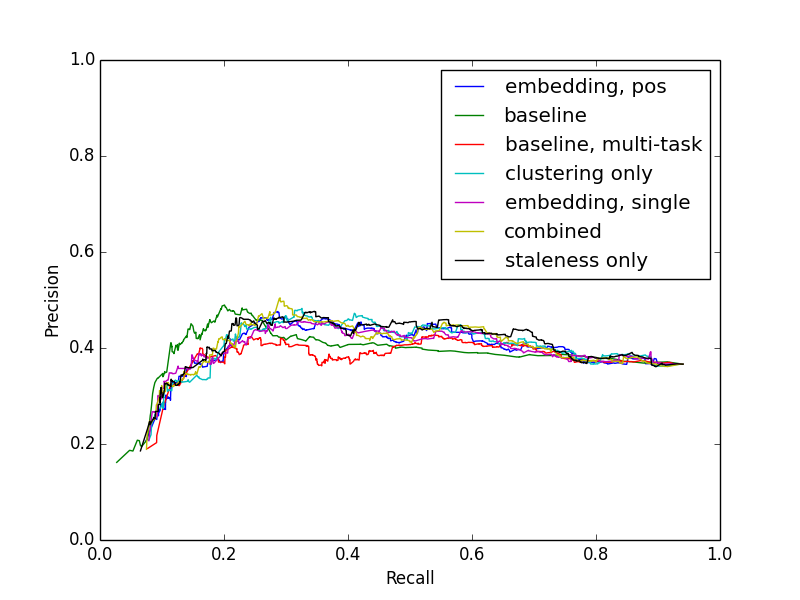
\includegraphics[width=.5\textwidth]{fig/macroPrecisionRecall.png}
\caption{Macro Precision-Recall}
\label{macroPrecRecall}
\end{figure}

\begin{figure}[tb]
\centering
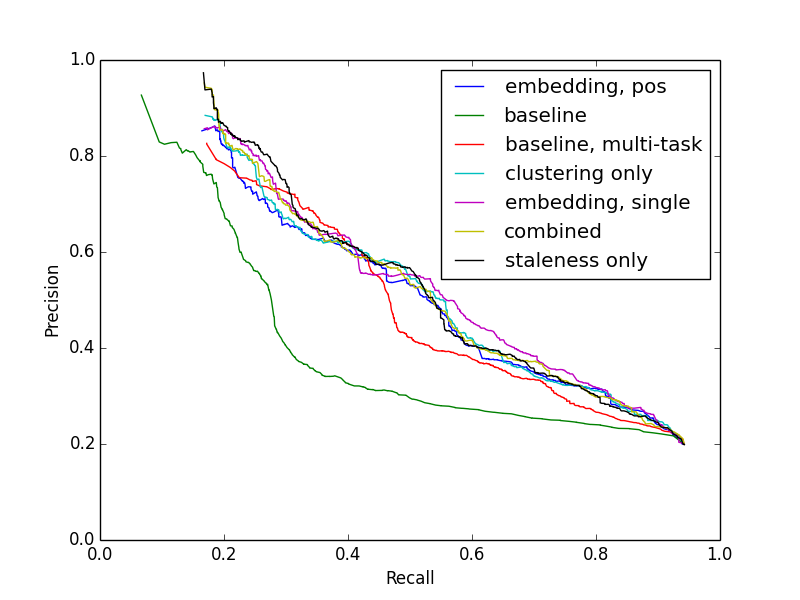
\includegraphics[width=.5\textwidth]{fig/microPrecisionRecall.png}
\caption{Micro Precision-Recall}
\label{microPrecRecall}
\end{figure}

Figures \ref{macroRuns} and \ref{microRuns} complement the revised results in Table \ref{officialRes} for different confidence cutoffs. Figures \ref{official:macroprec} and \ref{official:macrorecall} show that the macro recalls have a huge increase on the low confidence half of the plot, while most precisions stay nearly the same; this is a strong indicator of why the F1 boosts in the revised macro scenario.
In the micro case, the precisions and recalls (shown in Figures \ref{official:microprec} and \ref{official:microrecall}) increase and decrease in similar proportions, which explain why the micro revised F1s are almost the same as the micro official ones. 

Figures \ref{macroPrecRecall} and \ref{microPrecRecall} further illustrate the precision-recall for the different methods. In the macro case, all methods are pretty much the same. The micro metrics, in Figure \ref{microPrecRecall}, are much more interesting. On low recall, the micro precision of the different models meets our expectations, the more complex methods, which include non-parametric clustering and staleness, in general outperform the simpler ones. Nevertheless, on high recall, {\textit{Embedding Combined}} takes the lead.

%Table \ref{varyinggamma} shows the results for a variant of {\textit{Clustering Dynamic}}. As opposed to the {\textit{Clustering Dynamic}} in Table \ref{res}, this new version uses a single embedding representation instead of embeddings per word type. We show outputs using a low, medium and high $\gamma_i$, for $\alpha=0.$. We further perform a scan on a long range of $\gamma_d$ to see its impact on the overall result. 

%We achieve the best result when $\gamma_i=0.5$ and $\gamma_d=0.2$, still lower than \textit{Embedding Combined} but better than previous {\textit{Clustering Dynamic}}. In general, lower $\gamma_d$ seems to be doing a better job. These results further reflect the importance of hyperparameter tuning.

%Figure \ref{varyingalpha} shows the results for a variant of {\textit{Clustering Dynamic}}. As opposed to the {\textit{Clustering Dynamic}} in Table \ref{resMacro}, this new version uses a single embedding representation instead of embeddings per word type. We show the change in macro P-R-F1 for different values of $\alpha$, using $\gamma_{inc}=0.1$ and $\gamma_{dec}=1$. We see that the performance degrades as $\alpha$ increases, which further reflects the importance of hyperparameter tuning. Even more, this variant with $\alpha=0.2$ performed the best, achieving a macro F1 of 0.374.

%\begin{figure}[tb]
%\centering
%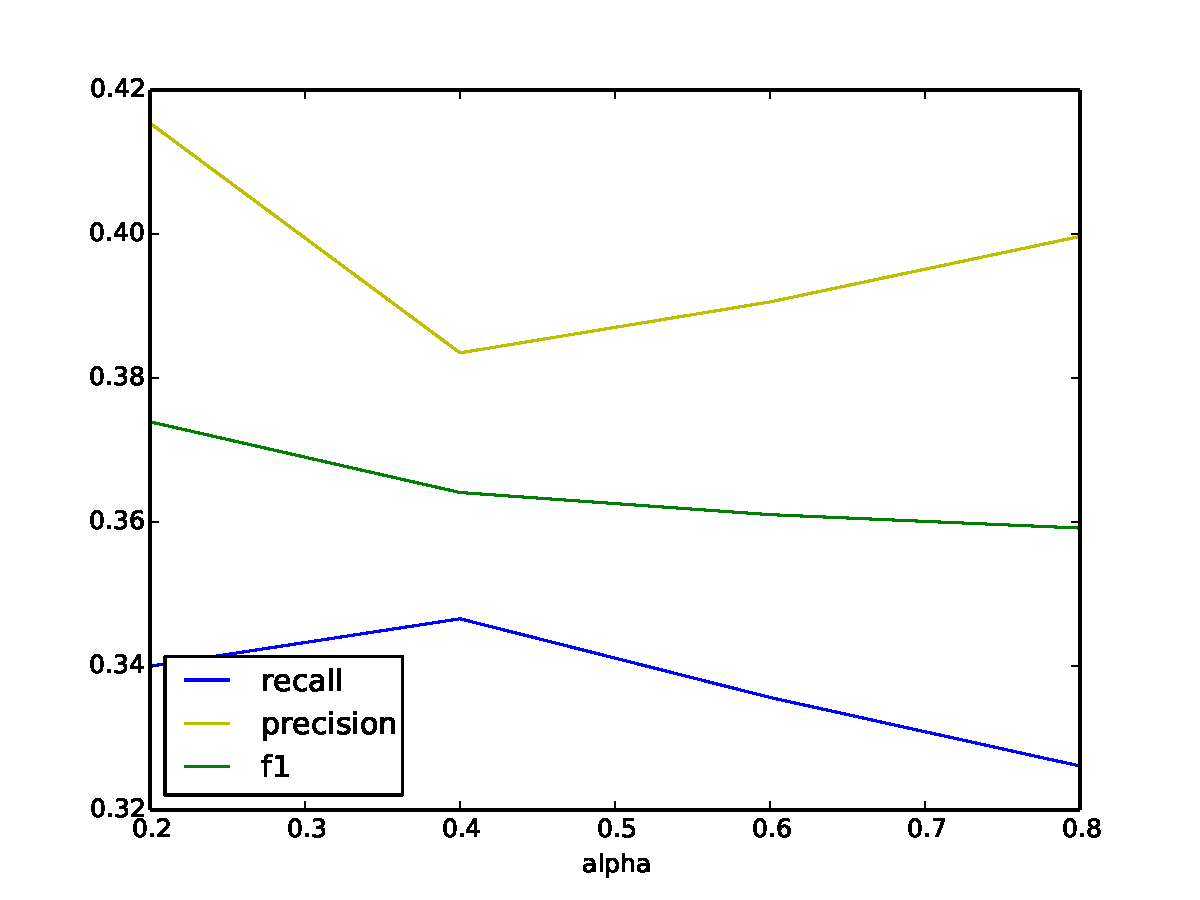
\includegraphics[width=0.8\columnwidth]{fig/alphaPlotMacro.pdf}
%\caption{P-R-F1 vs. $\alpha$}
%\label{varyingalpha}
%\end{figure}

%\begin{table}[tb]
%\center
%\begin{tabular}{cc}
%\toprule
%\textbf{C1} & \textbf{C2} \\
%\midrule
%Monday & conduct \\ %\hline
%Tuesday & complication \\ %\hline
%month & judicial \\ %\hline
%billion & government \\ %\hline
%million & guidance \\
%\bottomrule
%\end{tabular}
%\caption{Topic clusters closest words for \emph{Shawn Atleo}}
%\label{clusterresult}
%\end{table}

%Further, we present some qualitative results on the topic clusters of {\textit{Clustering Dynamic}} with a single embedding. Table \ref{clusterresult} illustrates the 5 closest words to the word that is most similar (in cosine similarity) to the cluster centroids of the entity \emph{Shawn Atleo} on 11/15/2012.
%By doing some manual search on \emph{Shawn Atleo}, we can easily confirm that C2 elements make sense. \emph{Mr. Atleo} is an activist for the rights of First Nations in Canada, and received several Honorary Doctorate of Laws degrees from different universities, which explains a cluster with the words in Table \ref{clusterresult}. C1 is somewhat harder, it is a cluster close to dates and finances. It may be explained by all the articles that talk about \emph{Shawn} announcing huge investments in different areas.

We believe further experimental investigations are needed to account for the correct tuning of the hyperparameters of the model. Exploiting external resources such as Wikipedia entity pages to construct more features \cite{xitong12} should probably increase the overall accuracy of our method. 

\section{Conclusion \& Future Work}
\label{conclusion}

Filtering streaming documents to accelerate users filling knowledge gaps plays a crucial role in the maintenance and update of knowledge bases.
With the exponential increase of information on the web, it becomes critical to detect relevant documents and incorporate their information to entities in a timely manner. % \cite{jingang13}.

In this paper we introduced a semi-supervised learning model for document filtering tasks. We proposed a distributed, non-parametric representation of documents suitable for streaming settings, that groups entities' references into topic clusters. Further, we present a notion of staleness computed per entity as well as per topic cluster, which dynamically estimates entities' and clusters' relevances.
Combining these three core ideas, distributed word embeddings, non-parametric clustering, and staleness, results in a more accurate representation of entities' contexts, and simultaneously addresses the filtering requirements of large corpora of streaming text documents.

Further work needs to be done. A possible line of future research would be exploring hierarchical clustering algorithms to better represent topic clusters. It would also be interesting to assess the effect of learning the hyperparameters of the model instead of just manual tuning them for the specific datasets.
It would also be worthwhile to assess the effects of using different pre-trained word embeddings.

\section*{Acknowledgments} 
 
This work was supported in part by the Argentine Ministry of Science, Technology and Productive Innovation with the program BEC.AR, and the TerraSwarm Research Center, supported by the STARnet phase of the Focus Center Research Program (FCRP). Any opinions, findings and conclusions or recommendations expressed in this material are those of the authors and do not necessarily reflect those of the sponsors.

%\newpage
\small
\bibliography{../kba}
\bibliographystyle{icml2014}

\end{document} 


